\documentclass[11pt, a4paper]{article}
\title{SPS : CW2 Report}
\author{Matthew Duffin}

\renewcommand\thesection{\arabic{section}}
\renewcommand\thesubsection{(\alph{subsection})}

\usepackage[linesnumbered,boxed]{algorithm2e}
\usepackage[margin=2cm]{geometry}
\usepackage{fancyhdr}
\usepackage{graphicx}
%\usepackage{subfig}
\usepackage{titling}

\usepackage{subcaption}

\setlength{\droptitle}{-60pt}

\pagestyle{fancy}
\fancyhf{}
\rhead{np14842, md14816}
\lhead{Nick Pearson, Matthew Duffin}
\cfoot{Page \thepage}

\begin{document}
\maketitle

\section{Introduction}
This report describes the process of desiging a classifier for a set of characters. By extracting features from the fourier space images of these three types of character (S, T and V) I have been able to build a reasonably accurate classifier. 

\section{Feature Selection}
The first step in the process is to find the features that clearly separate the three types of character. We were asked in this task to extract features from the fourier space. As a starting point I created the fourier space images for each of the characters and then took the average of each class. The results of this are shown below. 

\begin{figure}[ht]
\centering
	\begin{minipage}[b]{0.3\textwidth}
		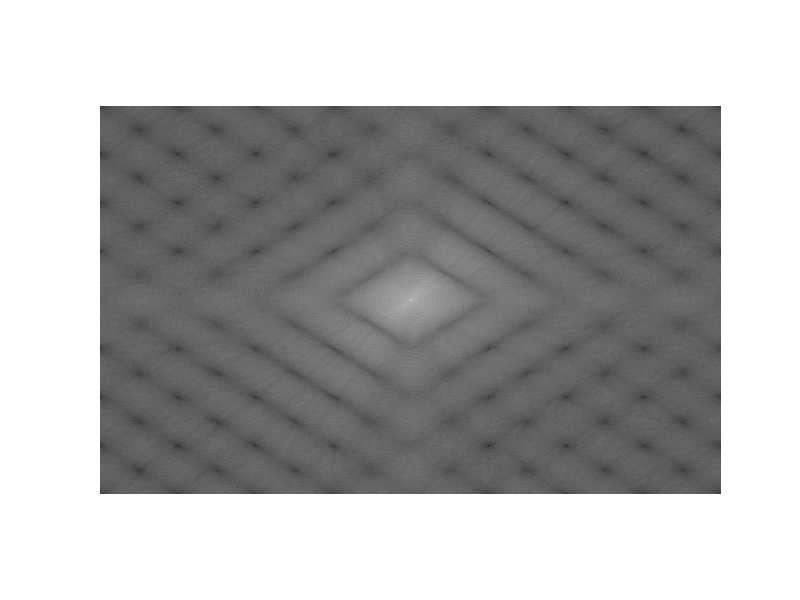
\includegraphics[trim={2cm 2cm 2cm 2cm},clip,width=0.8\textwidth]{characters/S_average.png}
	\end{minipage}	
	\begin{minipage}[b]{0.3\textwidth}
		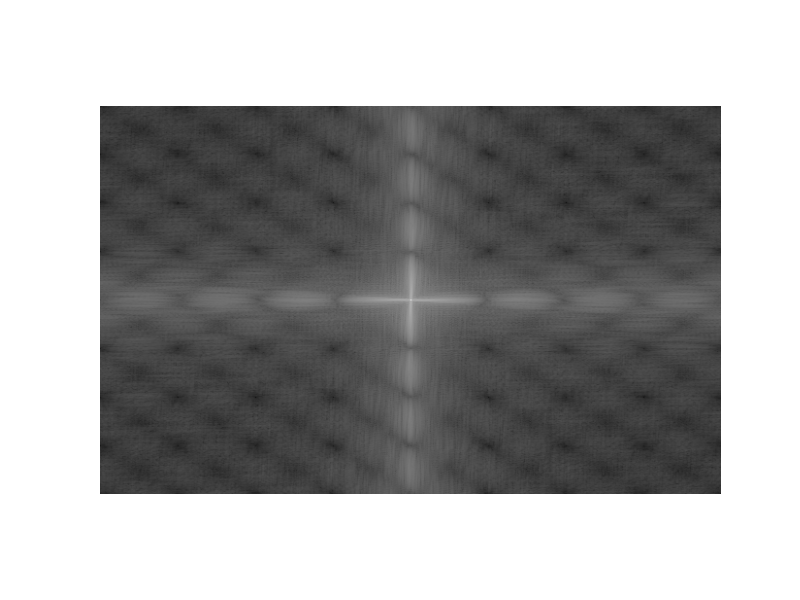
\includegraphics[trim={2cm 2cm 2cm 2cm},clip,width=0.8\textwidth]{characters/T_average.png}
	\end{minipage}
	\begin{minipage}[b]{0.3\textwidth}
		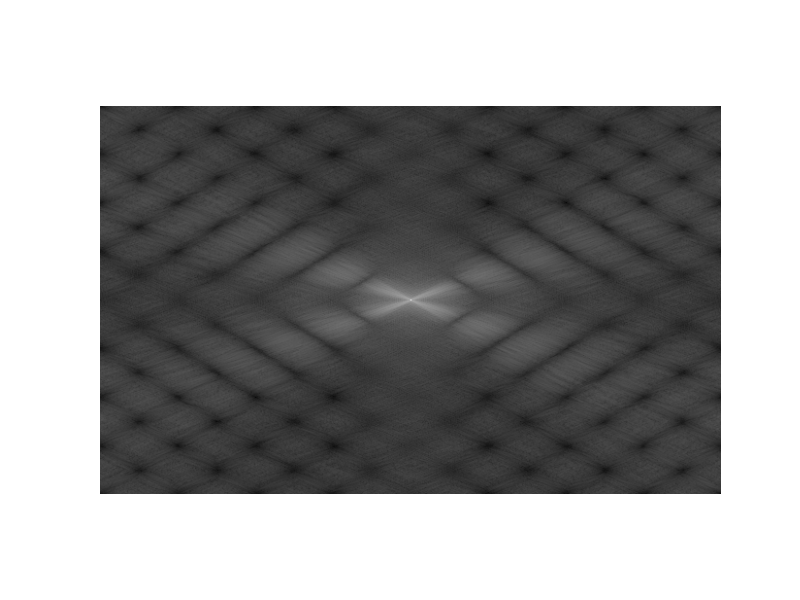
\includegraphics[trim={2cm 2cm 2cm 2cm},clip,width=0.8\textwidth]{characters/V_average.png}
	\end{minipage}
	\caption{Average fourier spaces of S (left) T (centre) and V (right).}
	\label{fig:averages}
\end{figure}

You can see that the fourier space for the letter T has very strong spectral peaks in the horizontal and vertical directions. The vertical line tells us that in the original image there is a high rate of change of intensity in the horizontal direction. The horizontal line shows the same for the vertical direction. Looking at the letter T you can indeed see that the two lines that make it up correspond to the strong bright vertical and horizontal lines in the fourier space. 

At this point I looked at the three images and tried to find regions where the intensity differed. For example, the strong horizontal and vertical lines that are present in the T fourier space are not present in the others. Likewise, the diagonal lines in V's fourier space are not present in the others. Using this information I selected five different regions to take forward and test, which can be seen in Figure ~\ref{fig:features}.

\begin{figure}[ht]
\centering
	\begin{minipage}[b]{0.3\textwidth}
		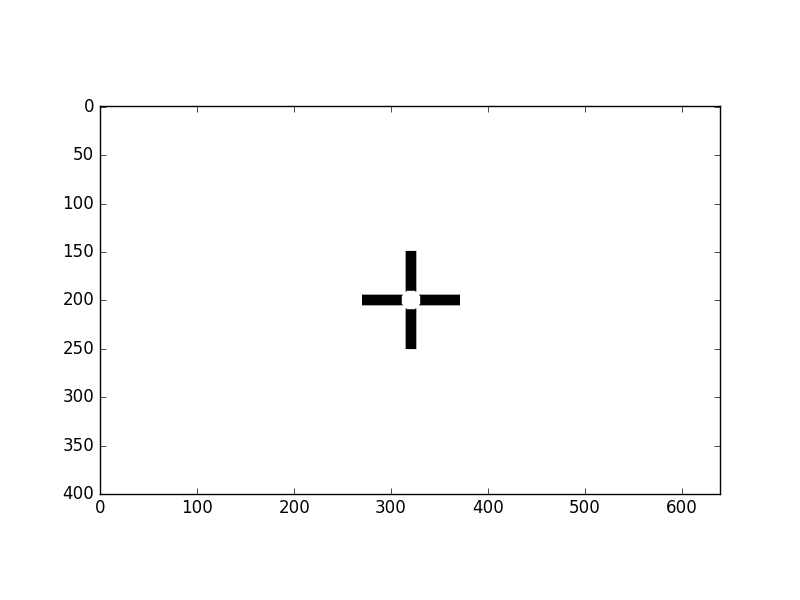
\includegraphics[trim={2cm 2cm 2cm 2cm},clip,width=0.8\textwidth]{features/cross.png}
	\end{minipage}	
	\begin{minipage}[b]{0.3\textwidth}
		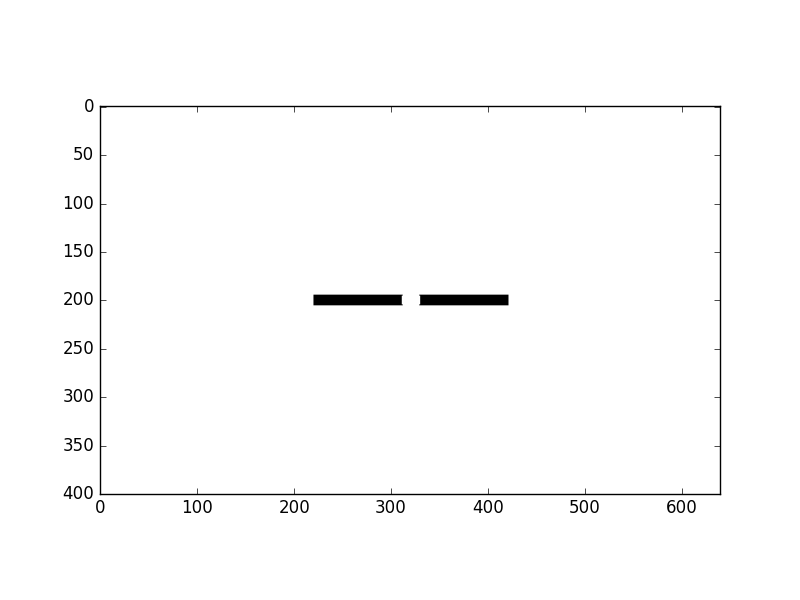
\includegraphics[trim={2cm 2cm 2cm 2cm},clip,width=0.8\textwidth]{features/line.png}
	\end{minipage}
	\begin{minipage}[b]{0.3\textwidth}
		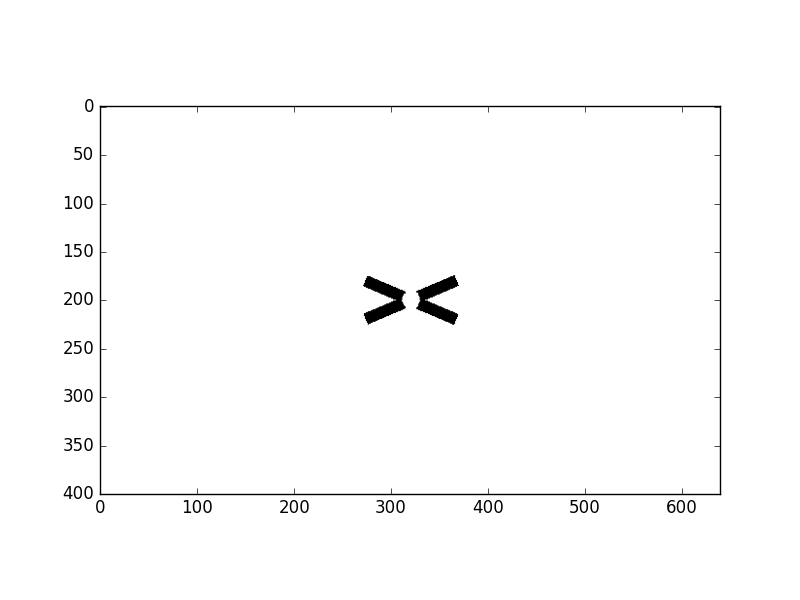
\includegraphics[trim={2cm 2cm 2cm 2cm},clip,width=0.8\textwidth]{features/x.png}
	\end{minipage}
	\begin{minipage}[b]{0.3\textwidth}
		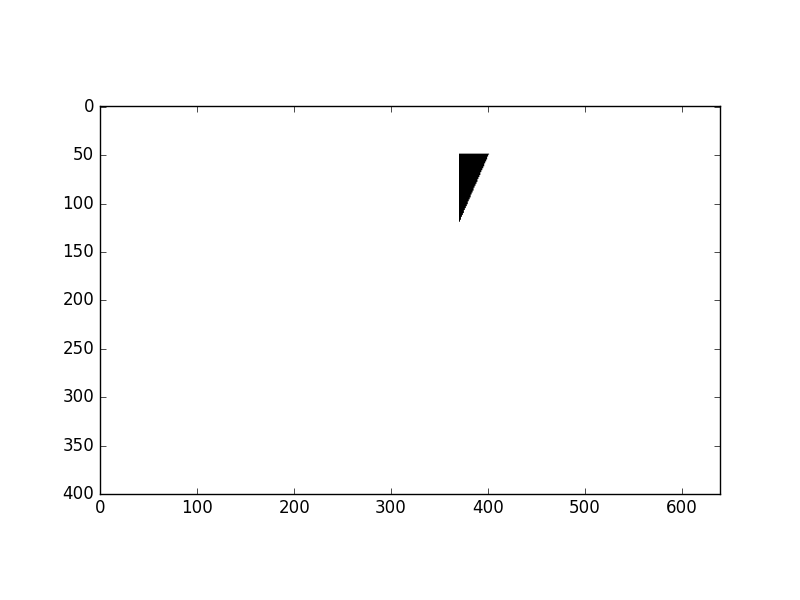
\includegraphics[trim={2cm 2cm 2cm 2cm},clip,width=0.8\textwidth]{features/triangle.png}
	\end{minipage}
	\begin{minipage}[b]{0.3\textwidth}
		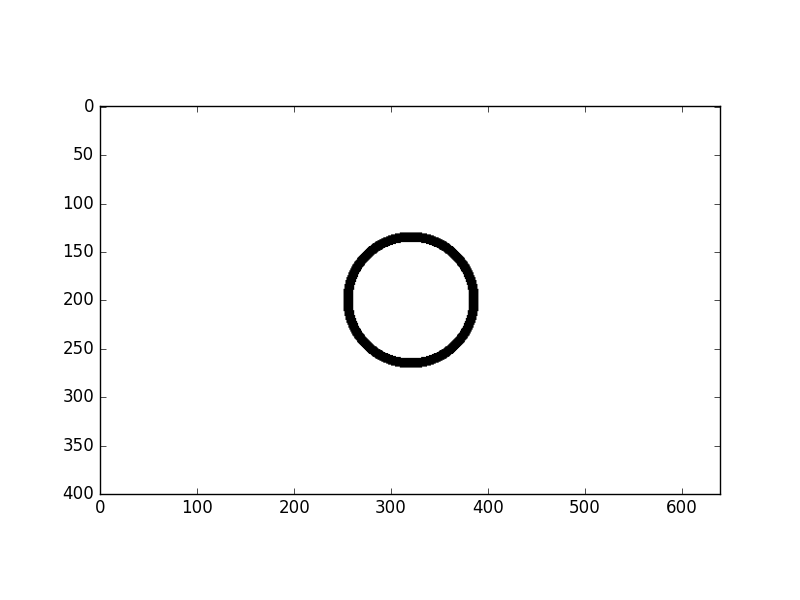
\includegraphics[trim={2cm 2cm 2cm 2cm},clip,width=0.8\textwidth]{features/ring.png}
	\end{minipage}
	\caption{Features selected to take forward to testing.}
	\label{fig:features}
\end{figure}
You will notice that a lot of the features have a "hole" in the middle. This is because I wanted to exclude the DC component from the features. The DC component is the average brightness of the image. It does not give any information about direction. Therefore its inclusion would be likely to skew my results if a certain image were brigher than the others. 
\begin{figure}[ht]
	\centering
	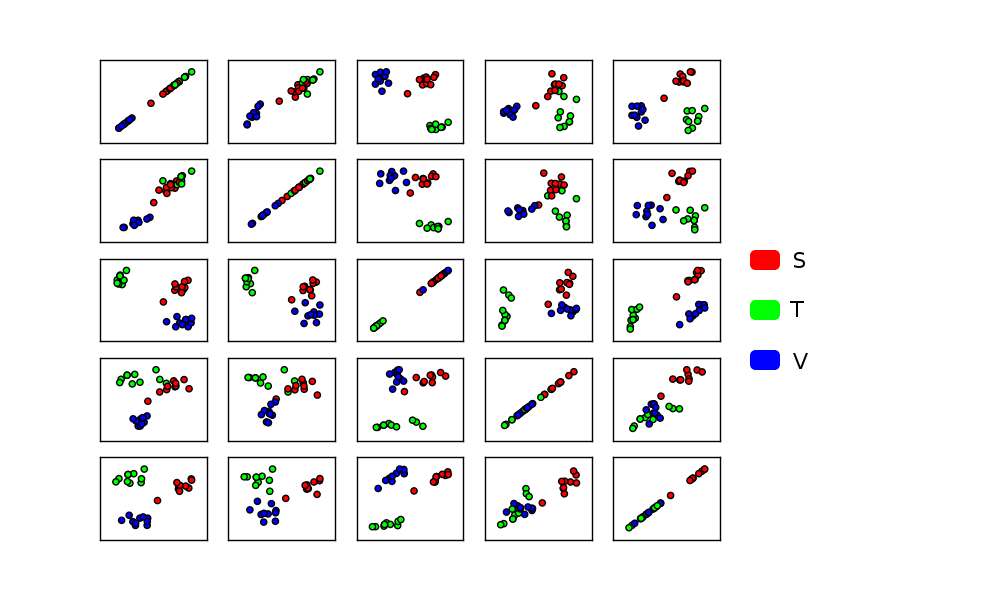
\includegraphics[trim={0 1.5cm 3cm 1.5cm},clip,width=0.75\textwidth]{feature_matrix_leg.png}
	\caption{A grid of plots, each of which plots one feature against another.}
	\label{fig:feature_matrix}
\end{figure}

Next, I took the log of the magnitude spectrum, squared it to get the power and then summed up the region defined by the feature.

In Figure ~\ref{fig:feature_matrix} I have plotted the features against each other to form a grid of plots. The features are numbered 0 to 4 downwards and 0 to 4 from left to right. There are a number of good candidates, such as (0,2) and (2,4) but I decided to take (0,4) forwards (the cross and the ring) because apart from one wayward point it separates the data into three well defined clusters. A more detailed plot of these two features can be seen in Figure ~\ref{fig:classifier_training}.



% The inter-cluster distance is high so there is a clear separation between clusters. The intra-cluster distances are low though so the underlying gaussian distributions for each cluster have low variance. 

\section{The Classifier}
\subsection{Training The Classifier}

\begin{figure}
\begin{minipage}[b]{.5\textwidth}
\centering
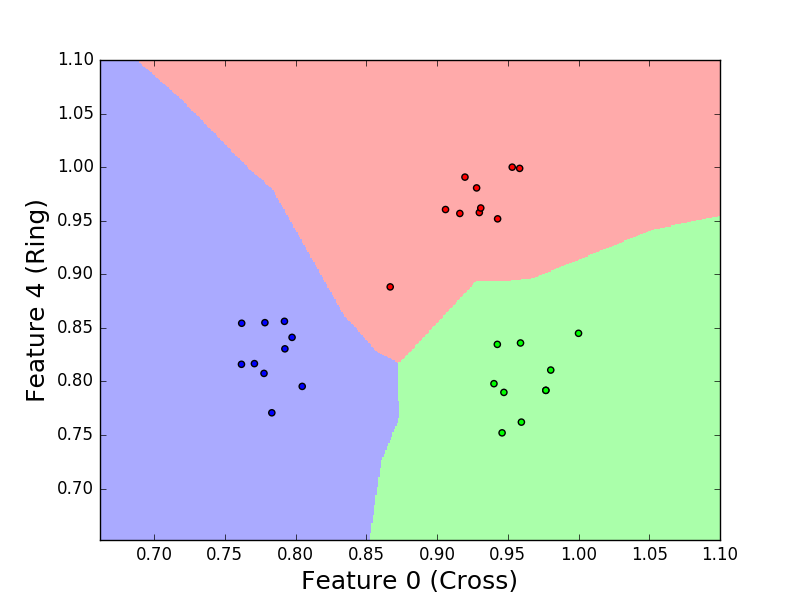
\includegraphics[width=1\textwidth]{training_plot_k1.png}
\subcaption{K=1}\label{fig:1a}
\end{minipage}%
\begin{minipage}[b]{.5\textwidth}
\centering
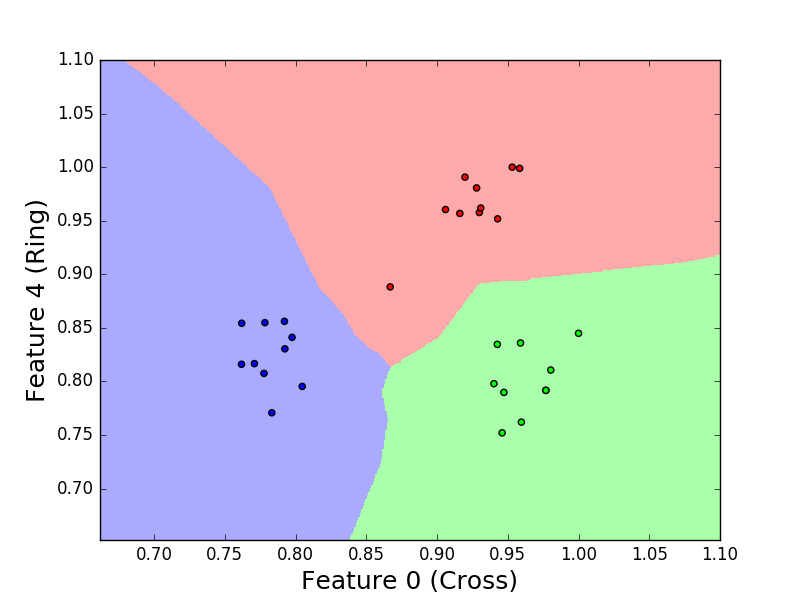
\includegraphics[width=1\textwidth]{training_plot_k2.png}
\subcaption{K=2}\label{fig:1a}
\end{minipage}
\begin{minipage}[b]{.5\textwidth}
\centering
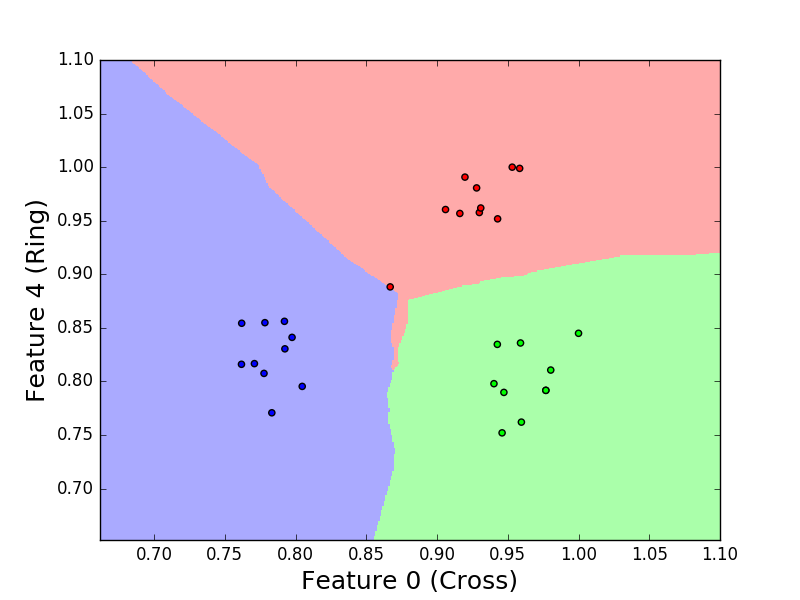
\includegraphics[width=1\textwidth]{training_plot_k3.png}
\subcaption{K=3}\label{fig:1b}
\end{minipage}%
\begin{minipage}[b]{.5\textwidth}
\centering
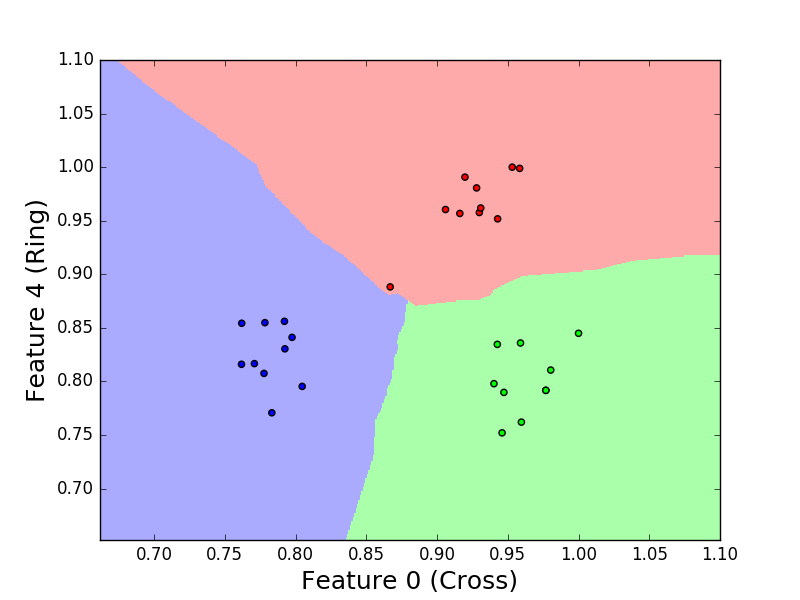
\includegraphics[width=1\textwidth]{training_plot_k4.png}
\subcaption{K=4}\label{fig:1b}
\end{minipage}
\caption{K-Nearest Neighbour Classifiers with K=1..4}\label{fig:1}
\end{figure}

%\begin{figure}[ht]
%\centering
%\begin{subfigure}[K=2]{%
%	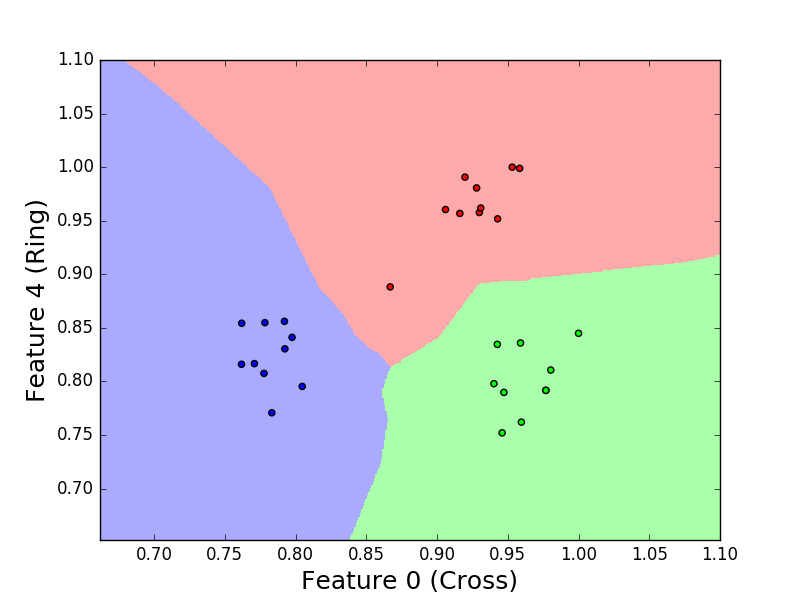
\includegraphics[]{training_plot_k2.png}
%	\label{fig:train_k2}}
%\quad
%\begin{subfigure}[K=3]{%
%	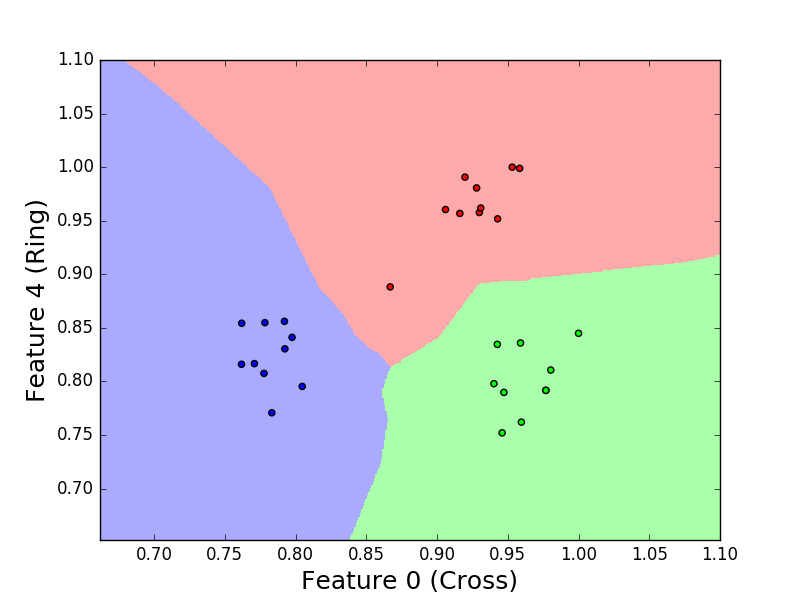
\includegraphics[]{training_plot_k2.png}
%	\label{fig:train_k3}}
%\quad
%\begin{subfigure}[K=4]{%
%	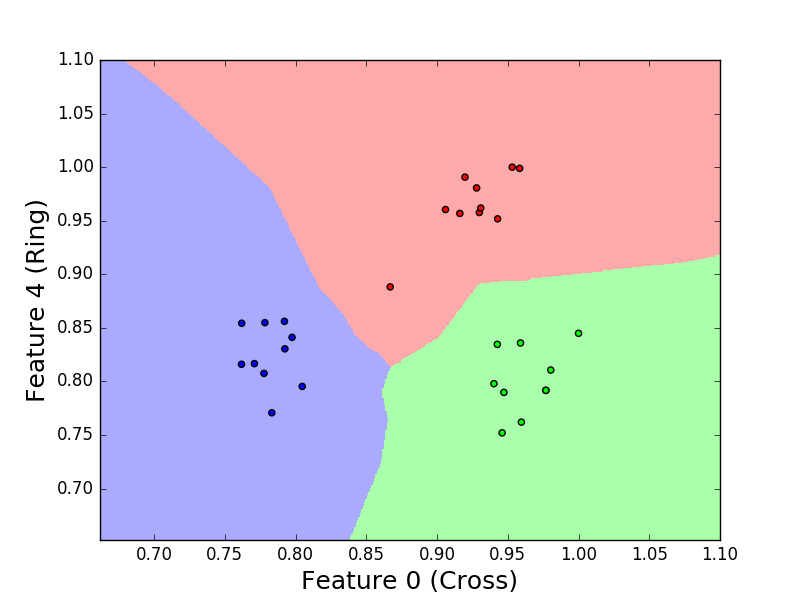
\includegraphics[]{training_plot_k2.png}
%	\label{fig:train_k4}}
%%
%\caption{The K-Nearest Neighbour classifier with K=2. The training data has also been plotted.}
%\label{fig:training_plots}
%\end{figure}

Figure ~\ref{fig:classifier_training} shows that the selection of features 0 and 4 was a good one. The K-Nearest Neighbours algorithm has produced a fairly well-defined decision boundary. Only one point sits right on the decision boundary between S and V. This is fine, as it shows we are avoiding over-fitting the model to the test data.

I must also mention that the values supplied to the K-Nearest Neighbour  algorithm were normalised first by dividing each feature by the largest value. This had no effect on the classification but just made the scale easier to interpret.

%During this stage we wanted to derive class labels for each data point. The first method  we used was the K-Means algorithm. At first we ran the algorithm until convergence to ensure that we did not recieve unusual results due to the random nature of initial centroid selection. As you can see from the graph, this worked very well, visually matching our expectations. The K-Means algorithm also returns the inertia. This is the sum of distances of data points to their closest centroid. For Nick's data the value is 163. Given there are 150 data points this means each point is on average roughly 1 unit from the closest centroid, which seems very good. 

\subsection{Testing The Classifier}

\begin{figure}[ht]
	\centering
	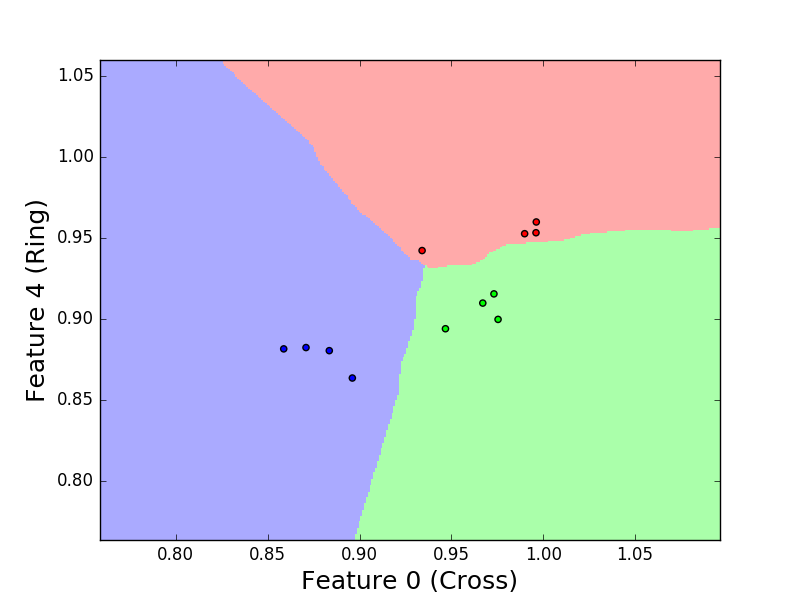
\includegraphics[trim={0 0 0 1cm},clip,width=0.75\textwidth]{test_plot.png}
	\caption{The K-Nearest Neighbour classifier with K=3. The test data has also been plotted.}
	\label{fig:classifier_test}
\end{figure}

\section{Nearest-Centroid Classification}
The next stage of our analysis was to start classifying new data. We started by using the centroids that we found using K-Means as a simple nearest-neighbour classifier. You can see the results in Figures ~\ref{fig:nearest_matt} and ~\ref{fig:nearest_nick}. The crosses represent the test data. As our features had high inter-cluster distance the nearest neighbour produced a fairly good assignment of data points. However, we could not test that it was getting the right result every time as we did not know which cluster each test point was \textit{supposed} to belong to.

%\begin{figure}[ht]
%\centering
%\begin{minipage}[b]{0.45\linewidth}
%	\includegraphics[trim={7cm 0 2cm 0},clip,width=1.1\textwidth]{nearest_matt.pdf}
%	\caption{Matt's data.}
%	\label{fig:nearest_matt}
%\end{minipage}
%%\quad
%\begin{minipage}[b]{0.45\linewidth}
%	\includegraphics[trim={7cm 0 2cm 0},clip,width=1.1\textwidth]{nearest_nick.pdf}
%	\caption{Nick's data.}
%	\label{fig:nearest_nick}
%\end{minipage}
%\end{figure}

% do you have any more to say here
%GRAPH HERE



\section{Maximum-Likelihood Classification}
Next we used a different classification method: maximum-likelihood classification (with each class modelled as being drawn from a 2-D Normal Distribution). This method has certain advantages over nearest-neighbour classification. In ML classification we need to estimate mean vectors as well as full covariance matrices for each class. This may result in a non-linear decision boundary if the covariance matrices are not the same across classes. \nocite{ml_wiki} \nocite{mvn_wiki}

Our first task was to plot contours around each cluster such that 95\% of the probability mass was inside the contour. We did this by finding the points where the squared Mahalanobis distance from the mean was 6. The Mahalanobis distance is a multi-dimensional measurement of how many standard deviations a point is from the mean \cite{mal_wiki}.

Next we plotted the decision boundaries. These allow us to classify future data as belonging to one of the three clusters. To generate these boundaries we found the points where the probabilities of belonging to cluster A's distribution and cluster B's distribution were equal.

%\begin{figure}[ht]
%\centering
%\begin{minipage}[b]{0.45\linewidth}
%	\includegraphics[trim={6cm 0 2cm 0},clip,width=1.1\textwidth]{contour_matt.pdf}
%	\caption{Matt's data.}
%	\label{fig:minipage7}
%\end{minipage}
%%\quad
%\begin{minipage}[b]{0.45\linewidth}
%	\includegraphics[trim={6cm 0 2cm 0},clip,width=1.1\textwidth]{contour_nick.pdf}
%	\caption{Nick's data.}
%	\label{fig:minipage8}
%\end{minipage}
%%\caption{The 15 test data points have been classified. They are shown by an 'x' and the training data by an 'o'.}
%\end{figure}

We then considered how you could change the maximum-likelihood classifier so that its decision boundaries were the same as the ones we found using the nearest-centroid method. We found that you can use the identity matrix as the covariance matrix for the two distributions instead of thier true covariances. This way there appears to be no correlation between the features within each cluster. Also, the two covariance matrices are identical. This creates a straight decision boundary that bisects the line between the two centroids.

%\begin{figure}[ht]
%\centering
%\begin{minipage}[b]{0.45\linewidth}
%	\includegraphics[trim={7cm 0 2cm 0},clip,width=1.1\textwidth]{prior_matt.pdf}
%	\caption{Matt's data.}
%	\label{fig:prior_matt}
%\end{minipage}
%%\quad
%\begin{minipage}[b]{0.45\linewidth}
%	\includegraphics[trim={7cm 0 2cm 0},clip,width=1.1\textwidth]{prior_nick.pdf}
%	\caption{Nick's data.}
%	\label{fig:prior_nick}
%\end{minipage}
%\end{figure}

We also experimented with adding a prior to one of the three classes. Figures ~\ref{fig:prior_matt} and ~\ref{fig:prior_nick} show how the decision boundaries change (dotted line) when one of the classes is twice as likely.

\section{Discussion}
In conclusion, we agreed that the decision boundaries we achieved would be sufficient to assign new data points to our clusters. The use of Maximum-Likelihood Classification would seem more accurate for deciding points which are near the decision boundary, as our clusters had different covariance values from one another. \\
The data we were given demonstrates how much information you can gain without any prior knowledge of where data was sourced. If we had more knowledge we could have used a MAP estimation for a final stage allowing for better results. However, we found that even giving one class a prior of 2 times the rest did not move the decision boundaries very far. This indicates that only a strong prior would affect classification greatly.

\section{Sources}
\renewcommand{\refname}{\vspace{-2em}}
\begin{thebibliography}{9}

\bibitem{mal_wiki}
  Mahalanobis Distance Wikipedia,
  https://en.wikipedia.org/wiki/Mahalanobis\_distance,
  Retrieved 11th March 2016.
  
\bibitem{ml_wiki}
  Maximum Likelihood Wikipedia,
  https://en.wikipedia.org/wiki/Maximum\_likelihood,
  Retrieved 11th March 2016.
  
\bibitem{mvn_wiki}
  Multivariate Normal Wikipedia,
  https://en.wikipedia.org/wiki/Multivariate\_normal\_distribution,
  Retrieved 11th March 2016.
  
\bibitem{km_wiki}
  K-Means Wikipedia,
  https://en.wikipedia.org/wiki/K-means\_clustering,
  Retrieved 11th March 2016.

\end{thebibliography}
\end{document}